\section{Daylighting Devices}\label{daylighting-devices}

Daylighting devices are used to improve daylighting in a zone.~ Besides their contribution to illuminance, daylighting devices also have a thermal impact on the zone heat balance.~ As a result the simulation of daylighting devices is tightly integrated into both the daylighting model and the zone heat balance.

There are two types of daylighting device in EnergyPlus:~ tubular daylighting devices and daylighting shelves.

\subsection{Tubular Daylighting Devices}\label{tubular-daylighting-devices}

The input object DaylightingDevice:Tubular provides a special model for fenestration components known as Tubular Daylighting Devices (TDDs), also known as tubular skylights or light pipes.~ TDDs are constructed of three components: a dome, a pipe, and a diffuser.

\begin{figure}[hbtp] % fig 66
\centering
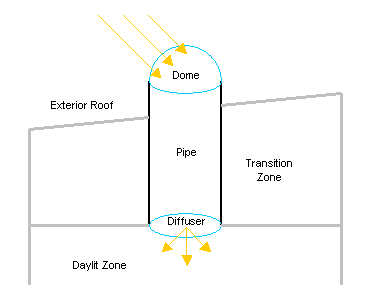
\includegraphics[width=0.9\textwidth, height=0.9\textheight, keepaspectratio=true]{media/image869.png}
\caption{Tubular Daylighting Devices \protect \label{fig:tubular-daylighting-devices}}
\end{figure}

The dome is typically a hemisphere made of clear plastic.~ It allows daylight into the pipe while keeping exterior weather out.~ The pipe is assumed to be a smooth cylinder with a highly reflective inside surface.~ The surface is usually either bare polished metal or a special reflective sheet adhered to the inside.~ The pipe channels the daylight from the dome to the diffuser via multiple internal reflections.~ The diffuser is typically a flat frosted plastic cover.~ The diffuser evenly distributes the daylight to the zone.~ The dome/diffuser area and pipe area must be approximately equal (within 2\%) for running the simulation successfully.

In EnergyPlus the TDD model includes three different, but related, phenomena:

\begin{itemize}
\item
  Daylighting
\item
  Solar gains
\item
  Conductive/convective gains
\end{itemize}

Solar gains and conductive/convective gains are simulated by the zone heat balance.~ Daylighting is simulated independently.

For both daylighting and heat balance simulations, the dome and diffuser are treated as special window surfaces to take advantage of many of the standard daylighting and heat transfer routines.~ Together the dome and diffuser become ``receiver'' and ``transmitter'', i.e.~radiation entering the dome ends up exiting the diffuser.

\begin{figure}[hbtp] % fig 67
\centering
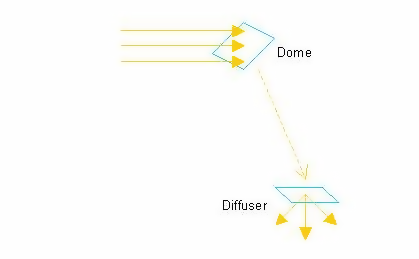
\includegraphics[width=0.9\textwidth, height=0.9\textheight, keepaspectratio=true]{media/image870.png}
\caption{Dome and Diffuser Surfaces \protect \label{fig:dome-and-diffuser-surfaces}}
\end{figure}

The pipe is simulated by a separate code module.~ While several different measures for characterizing TDD performance are in use (Zhang 2002; Harrison 1998), the total transmittance of the TDD is most compatible with the EnergyPlus daylighting and heat balance code.~ Calculation of the transmittance of the pipe and the TDD for different types of radiation is fundamental to all phenomena covered by the model.

\subsubsection{Pipe Beam Transmittance}\label{pipe-beam-transmittance}

The transmittance of beam radiation is derived from the integration of the transmittance of many discrete rays.~ The transmittance of a discrete ray through a pipe is dependent on the reflectivity of the inside pipe surface, the aspect ratio of the pipe, the incident angle of the ray, and the point of entry into the pipe.

\begin{figure}[hbtp] % fig 68
\centering
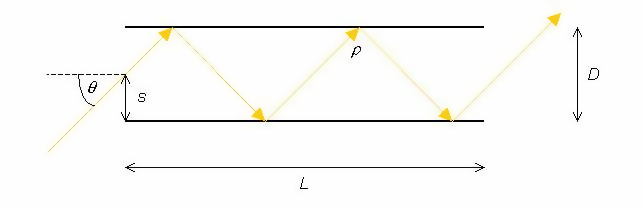
\includegraphics[width=0.9\textwidth, height=0.9\textheight, keepaspectratio=true]{media/image871.png}
\caption{Discrete Ray in a Pipe \protect \label{fig:discrete-ray-in-a-pipe}}
\end{figure}

For an opaque surface, the reflectivity is:

\begin{equation}
\rho  = 1 - \alpha
\end{equation}

where \(\alpha\) = surface absorptivity.~ Visible (i.e.~daylighting) and solar absorptivities give visible and solar reflectivities, respectively.~ Measured reflectivities for commercial TDDs range from 0.90 to 0.99.~ Although the actual surface reflectivity is slightly dependent on the incident angle, the model assumes a constant reflectivity for all angles.

The full analytical expression for the transmittance of a beam of light in a highly reflective pipe has been developed by Swift and Smith and verified by experiment (1994).~ By integrating over all rays incident on the pipe entrance, they find the transmittance of a beam of collimated radiation to be:

\begin{equation}
\tau  = \frac{4}{\pi }\int_{s = 0}^1 {\frac{{{s^2}}}{{\sqrt {1 - {s^2}} }}} {\rho ^{INT\left[ {a\tan \theta /s} \right]}}\left( {1 - \left( {1 - \rho } \right)\left( {a\tan \theta /s - INT\left[ {a\tan \theta /s} \right]} \right)} \right)ds
\end{equation}

where

a = L/D, the aspect ratio of the TDD

\(\rho\) = surface reflectivity

\(\theta\) = incident angle

s = entry point

This integral does not have an analytical solution and must be calculated numerically.~ It was found that a large number of points (100,000) were necessary to achieve an acceptable accuracy.~ Since the integration is time consuming and the transmittance of the pipe must be utilized many times at every time step, values are calculated over a range of incident angles and stored in a table.~ The tabulated values are interpolated to rapidly give the transmittance at any incident angle.~ A polynomial fit was also considered but it was found that interpolation gave superior results.

In the graph below, interpolated values from EnergyPlus are compared to the results of ray tracing simulations performed at the Florida Solar Energy Center for an incident angle of 30 degrees (McCluney 2003).

\begin{figure}[hbtp] % fig 69
\centering
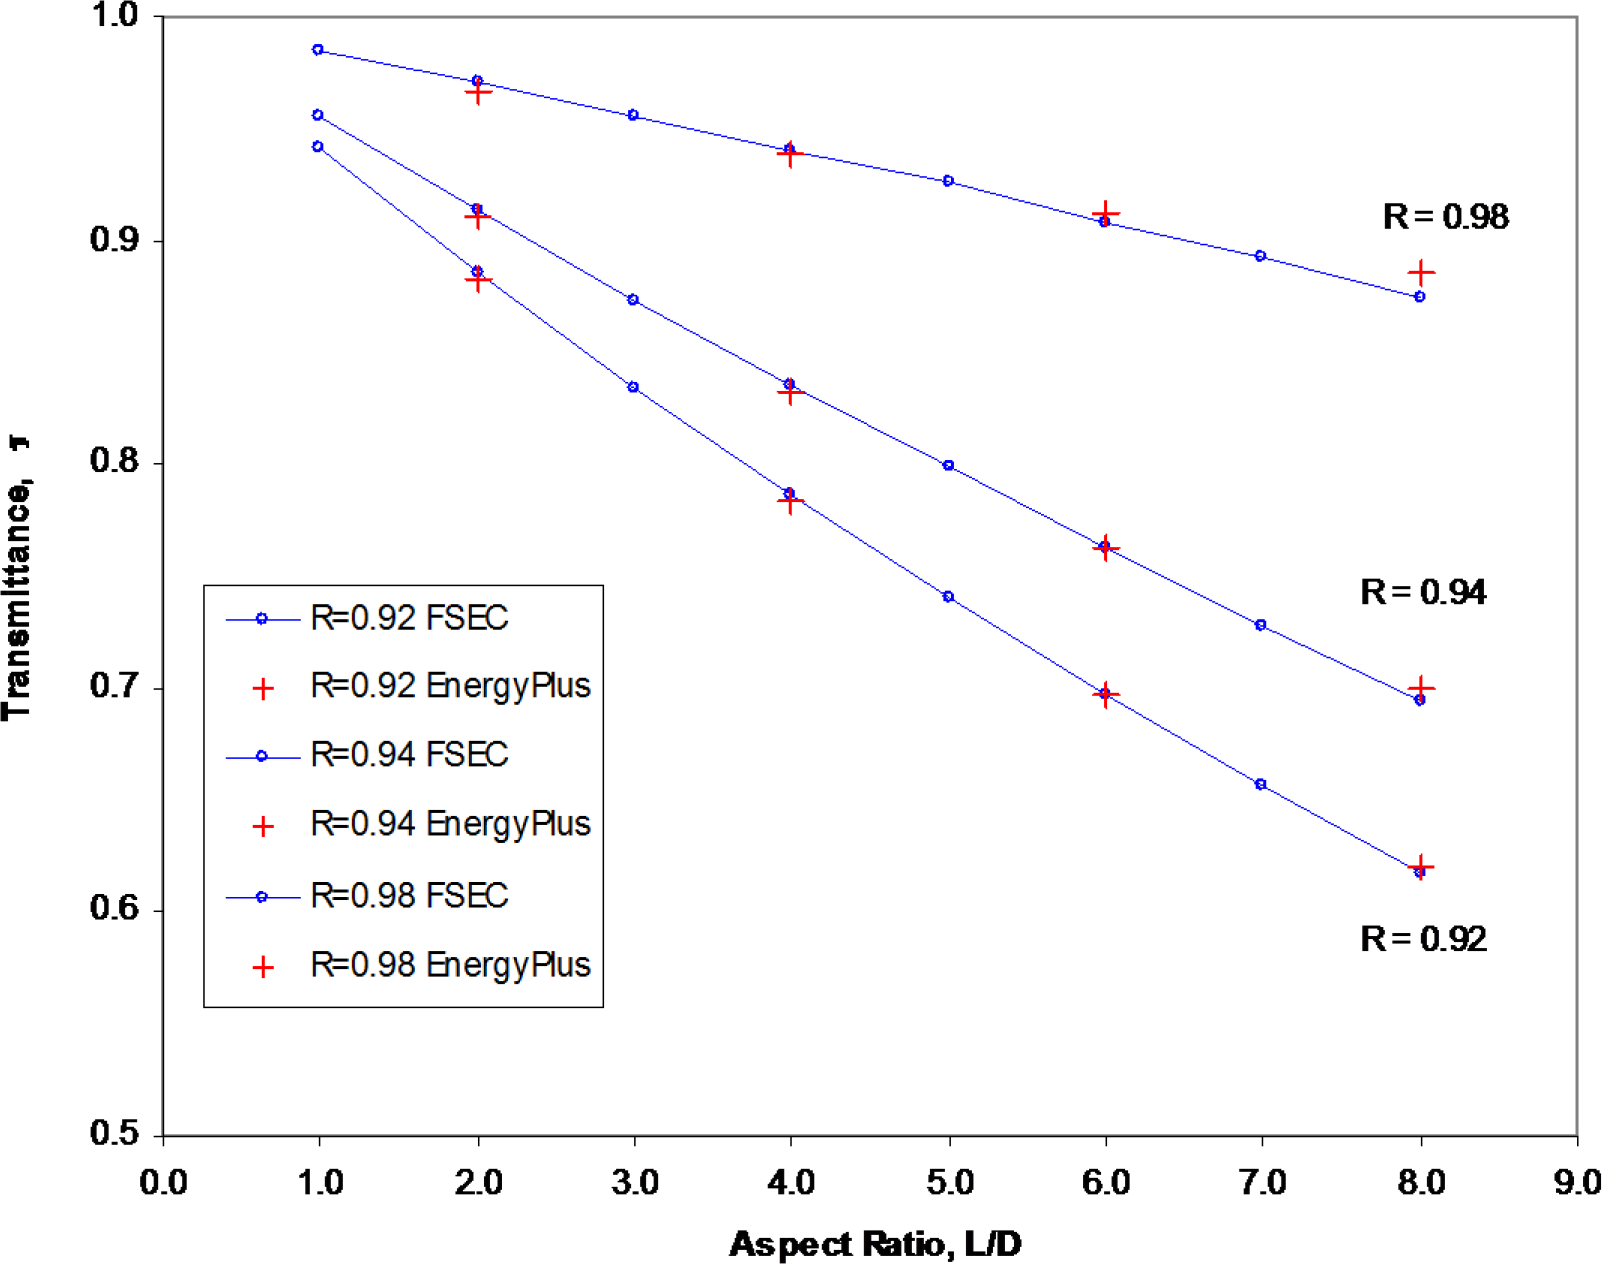
\includegraphics[width=0.9\textwidth, height=0.9\textheight, keepaspectratio=true]{media/image874.png}
\caption{Pipe Transmittance Comparison. \protect \label{fig:pipe-transmittance-comparison.}}
\end{figure}

During initialization of each unique TDD, the program integrates and tabulates values for the visible and solar transmittance of the pipe.~ The results are subsequently used in the daylighting simulation and heat balance simulation respectively.

The effect of bends in the pipe on beam transmittance is not included in this model.~ Recent research (Zhang 2002) has suggested that a 30 degree bend has a 20\% loss in transmitted light.~ If the effect of bends must be simulated, it can be approximated by the user by appropriately decreasing the transmittance of the diffuser material.

\subsubsection{TDD Beam Transmittance}\label{tdd-beam-transmittance}

The beam transmittance of the TDD takes into account the dome and diffuser transmittances in addition to the pipe transmittance.

\begin{equation}
{\tau_{TDD}}(\theta ) = {\tau_{dome}}(\theta ){\tau_{pipe}}(\theta ){\tau_{diffuser}}
\end{equation}

where

\(\tau_{dome}\)(\(\theta\)) = beam transmittance of the dome glazing at the incident angle

\(\tau_{pipe}\)(\(\theta\)) = beam transmittance of the pipe at the incident angle, as described above

\(\tau_{diffuser}\) = diffuse transmittance of the diffuser glazing

The dome transmittance is calculated for a flat window.~ The model does not take into account refraction due to the curvature of the dome surface.

Diffuse transmittance is always assumed for the diffuser because multiple internal reflections in the pipe scatter the beam with a diffusing effect.~ Although the light exiting the pipe is not isotropic, it can be approximated as diffuse.~ The use of a frosted diffuser on the TDD, however, ensures that the light delivered to the zone is very close to isotropic diffuse.

The calculation of TDD diffuse transmittance is considerably more complex and is handled differently in the daylighting simulation and the heat balance simulation.~ The details are discussed in the following sections.

\subsubsection{Daylighting}\label{daylighting}

The daylighting simulation of the TDD treats the diffuser surface as a regular window illuminated from the outside by sun, sky, and ground.~ However, the TDD model replaces the window glazing transmittance with the appropriate TDD transmittance and converts all transmitted light to diffuse.

The illuminance due to the direct beam of the sun is found using the TDD beam transmittance t\(_{TDD}\)(\(\theta\)) as described above.~ The incident angle \(\theta\) is relative to the dome surface.

The illuminance due to sky radiation and ground reflected radiation is calculated with the normal daylighting model integration over the sky and ground within the viewable hemisphere of the dome.~ The transmittance of each sky or ground~ element is also found using the TDD beam transmittance at the incident angle of the sky or ground element relative to the dome.

Light from the diffuser is converted to diffuse inside the zone in the same way as an interior shade.

\subsubsection{Solar Gains}\label{solar-gains}

Solar radiation incident on a window is calculated separately as sun, sky, and ground radiation.~ A different transmittance must be applied for each type of radiation.

For beam radiation the TDD beam transmittance t\(_{TDD}\)(\(\theta\)) for the solar spectrum is used as described above.~ For sky and ground radiation a diffuse transmittance for the TDD must be developed.

The transmittance of diffuse radiation can be defined as the total transmitted flux divided by the total incident flux.

\begin{equation}
{\tau_{diff}} = \frac{{\sum {{I_{trans}}} }}{{\sum {{I_{inc}}} }}
\end{equation}

Swift and Smith (1994) suggest a weighted integral of the beam transmittance over the hemisphere for an arbitrary angular distribution:

\begin{equation}
{\tau_{diff}} = \frac{{\int_{\theta  = 0}^{\pi /2} {\tau (\theta )P(\theta )} \sin \theta d\theta }}{{\int_{\theta  = 0}^{\pi /2} {P(\theta )} \sin \theta d\theta }}
\end{equation}

where

P(\(\theta\)) = angular distribution function

For isotropic diffuse radiation P(\(\theta\)) is the cosine of the incident angle \(\theta\).

\begin{equation}
{\tau_{diff,iso}} = \frac{{\int_{\theta  = 0}^{\pi /2} {\tau (\theta )\cos \theta } \sin \theta d\theta }}{{\int_{\theta  = 0}^{\pi /2} {\cos \theta } \sin \theta d\theta }}
\end{equation}

For a given pipe or TDD, t\(_{diff,iso}\) is a constant.~ The program calculates t\(_{diff,iso}\) once during initialization using a numerical integration.

The diffuse isotropic transmittance is useful, but not sufficient, for determining the transmittance of sky radiation.~ As described in the \emph{Sky Radiance Model} section, sky radiation has an anisotropic distribution modeled as the superposition of three simple distributions: a diffuse isotropic background, a circumsolar brightening near the sun, and a horizon brightening.~ While the daylighting model is capable of calculating the luminance of any position in the sky, the solar code only calculates the ultimate irradiance on a surface.~ For this reason it is not possible to integrate over an angular distribution function for sky radiance.~ Instead the three sky distributions must be handled piecewise.

\begin{equation}
{\tau_{diff,aniso}} = \frac{{\sum {{I_{trans,aniso}}} }}{{\sum {{I_{inc,aniso}}} }} = \frac{{{I_{trans,iso}} + {I_{trans,circumsolar}} + {I_{trans,horiz}}}}{{{I_{inc,iso}} + {I_{inc,circumsolar}} + {I_{inc,horiz}}}}
\end{equation}

Substituting in the appropriate transmittances:

\begin{equation}
{\tau_{diff,aniso}} = \frac{{{\tau_{diff,iso}}{I_{inc,iso}} + \tau (\theta ){I_{inc,circumsolar}} + {\tau_{diff,horiz}}{I_{inc,horiz}}}}{{{I_{inc,iso}} + {I_{inc,circumsolar}} + {I_{inc,horiz}}}}
\end{equation}

where

\(\tau_{diff,iso}\) = diffuse isotropic transmittance

t(\(\theta\)) = beam transmittance at incident angle q of sun

\(\tau_{diff,horiz}\) = diffuse transmittance of the horizon, derived below

It is important to note that transmittances above are for the total TDD.~ The transmittance of the dome and diffuser must be included to account for their angular dependencies as well.

The beam transmittance is used as an approximation for all circumsolar radiation.

The diffuse horizon transmittance is found by integrating the beam transmittance over the arc of the horizon.

\begin{equation}
{\tau_{diff,horiz}} = \frac{{\sum {{I_{trans,horiz}}} }}{{\sum {{I_{inc,horiz}}} }} = \frac{{\int_{\theta  =  - \pi /2}^{\pi /2} {\tau (\theta )\cos \theta d\theta } }}{{\int_{\theta  =  - \pi /2}^{\pi /2} {\cos \theta d\theta } }}
\end{equation}

Since the radiance of the horizon is isotropic, and therefore constant across the entire horizon, the actual value of the radiance cancels out.~ The result is a constant that is calculated once during initialization.

Ground radiation is assumed to be isotropic diffuse.~ The transmittance of ground radiation is the diffuse isotropic transmittance.

\begin{equation}
{\tau_{diff,gnd}} = {\tau_{diff,iso}}
\end{equation}

The solar flux transmitted by a TDD due to beam, sky, and ground radiation is calculated as normal for a window but uses the respective transmittances for the TDD.

\begin{equation}
{q''_{TDD - trans,beam}} = \left( {{I_{sun}}\cos \theta } \right){f_{sunlit}}{\tau_{TDD}}(\theta )
\end{equation}

\begin{equation}
{q''_{TDD - trans,sky}} = {I_{h,sky}}{f_{skymult}}{\tau_{TDD,diff,aniso}}
\end{equation}

\begin{equation}
{q''_{TDD - trans,gnd}} = \left( {{I_{sun}}\cos \theta  + {I_{h,sky}}} \right){F_{sg}}{\tau_{TDD,diff,iso}}
\end{equation}

where

I\(_{sun}\) = solar beam intensity of the sun

I\(_{h,sky}\) = total horizontal diffuse solar radiation due to the sky

\(\theta\) = incident angle of the beam on the dome

f\(_{sunlit}\) = sunlit beam fraction of the dome area

f\(_{skymult}\) = anisotropic sky view multiplier (see AnisoSkyMult)

F\(_{sg}\) = view from ground to dome

\(\tau_{TDD}\)(\(\theta\)) = TDD beam transmittance

\(\tau_{TDD,diff,aniso}\) = TDD anisotropic sky transmittance

\(\tau_{TDD,diff,iso}\) = TDD isotropic diffuse transmittance

\subsubsection{Daylighting vs.~Solar}\label{daylighting-vs.solar}

The beam transmittance of a TDD is calculated in the same way for both daylighting and solar gains.~ If the visible and solar properties (i.e.~absorptances in the input file) are the same, the reported TDD beam transmittances are equal.

However, because the daylighting and solar models treat diffuse radiation differently, the TDD diffuse transmittances reported for visible and solar radiation will not necessarily be equal, even though the properties may be the same.

Since the daylighting model calculates the diffuse illuminance using a sky and ground integration of many discrete elements, a visible diffuse transmittance is not required for the TDD daylighting simulation.~ For reporting purposes only, the visible diffuse transmittance is estimated concurrent with the sky and ground integration using:

\begin{equation}
{\tau_{diff}} = \frac{{\int {{\tau_{TDD}}(\theta )d{\Phi_{inc}}} }}{{\int {d{\Phi_{inc}}} }}
\end{equation}

\subsubsection{Conductive/Convective Gains}\label{conductiveconvective-gains}

For conductive and convective heat gain, TDDs are treated as one entity with an effective thermal resistance (i.e.~R-value) between the outside and inside surfaces.~ The outside face temperature of the dome and the inside face temperature of the diffuser are calculated as usual by the outside and inside heat balances respectively.~ The temperatures are then copied to the inside face of the dome and the outside face of the diffuser.~ Normal exterior and interior convection and IR radiation exchange occurs for both surfaces.

Although little research has been done on the thermal characteristics of TDDs, one experiment (Harrison 1998) reports an average effective thermal resistance of 0.279 m\(^{2}\) K/W for a commercial TDD measuring 0.33 m in diameter by 1.83 m in length.~ This value, however, reflects a measurement from outdoor air temperature to indoor air temperature.~ The model assumes an effective thermal resistance from outside surface temperature to inside surface temperature.

Solar radiation is inevitably absorbed by the TDD before it reaches the zone.~ Every reflection in the pipe leaves behind some solar radiation according to the surface absorptance.~ Rays incident at a greater angle make more reflections and leave behind more absorbed solar in the pipe wall.

The total absorbed solar radiation in the TDD is the sum of the following gains:

\begin{itemize}
\item
  Inward bound solar absorbed by multiple pipe reflections
\item
  Outward bound solar absorbed by multiple pipe reflections due to: reflection off of diffuser surface (inside of TDD) and zone diffuse interior shortwave incident on the diffuser from lights, etc.
\item
  Inward flowing absorbed solar in dome and diffuser glazing
\end{itemize}

\begin{equation}
{Q_{abs,pipe}} = {Q_{abs,in}} + {Q_{abs,out}} + {Q_{abs,glazing}}
\end{equation}

The inward bound solar absorbed by the pipe is the difference between the solar transmitted by the dome and the solar incident on the diffuser.

\begin{equation}
{Q_{abs,in}} = {q''_{trans,dome}}{A_{dome}} - {q''_{inc,diffuser}}{A_{diffuser}}
\end{equation}

The solar transmitted by the dome q''\(_{trans,dome}\) is calculated as usual for a window.~ The solar incident on the diffuser q''\(_{inc,diffuser}\) is more complicated because each component must be treated separately.

\begin{equation}
{q''_{inc,diffuser}} = {q''_{beam}}\frac{{{\tau_{TDD,beam}}(\theta )}}{{{\tau_{diffuser}}}} + {q''_{sky}}\frac{{{\tau_{TDD,aniso}}(Hour)}}{{{\tau_{diffuser}}}} + {q''_{gnd}}\frac{{{\tau_{TDD,iso}}}}{{{\tau_{diffuser}}}}
\end{equation}

The outward bound solar absorbed by the pipe is given by:

\begin{equation}
{Q_{abs,out}} = \left( {{{q''}_{refl,diffuser}}\frac{{\left( {1 - {\tau_{TDD}}} \right)}}{{{\tau_{diffuser}}}} + {{q''}_{zoneSW}}\left( {1 - {\tau_{TDD}}} \right)} \right){A_{diffuser}}
\end{equation}

where q''\(_{zoneSW}\) is the zone interior diffuse shortwave flux from window, lights, and ambient surface reflections, and

\begin{equation}
{q''_{refl,diffuser}} = {q''_{inc,diffuser}} - {q''_{abs,diffuser}} - {q''_{trans,diffuser}}
\end{equation}

The inward flowing portion of solar absorbed in the dome and diffuser glazing is:

\begin{equation}
{Q_{abs,glazing}} = \frac{{{{q''}_{abs,dome}}{A_{dome}}}}{2} + \frac{{{{q''}_{abs,diffuser}}{A_{diffuser}}}}{2}
\end{equation}

All absorbed solar radiation in the TDD is distributed among the transition zones that the pipe passes through between dome and diffuser.~ The transition zone heat gain is proportional to the length of the zone.~ Any exterior length of pipe also receives a proportional amount of heat, but this is lost to the outside.

\subsubsection{References}\label{references-016}

Harrison, S. J., McCurdy, G. G., Cooke, R. 1998.~ ``Preliminary Evaluation of the Daylighting and Thermal Performance of Cylindrical Skylights'', Proceedings of International Daylight Conference, Ottawa, Canada, pp.~205-212.

McCluney, R. 2003. ``Rating of Tubular Daylighting Devices for Visible Transmittance and Solar Heat Gain -- Final Report'', FSEC-CR-1385-03, January 15, 2003, Florida Solar Energy Center, 1679 Clearlake Rd., Cocoa, FL 32922.

Swift, P. D., and Smith, G. B. 1995. ``Cylindrical Mirror Light Pipes'', Solar Energy Materials and Solar Cells 36, pp.~159-168.

Zhang, X., Muneer, T., and Kubie, J. 2002.~ ``A Design Guide For Performance Assessment of Solar Light-Pipes'', Lighting Research \& Technology 34, 2, pp.~149-169.

\subsection{Daylighting Shelves}\label{daylighting-shelves}

The input object DaylightingDevice:Shelf provides a special model for light shelves used to augment daylighting.~ Light shelves are constructed from up to three components: a window, an inside shelf, and an outside shelf.~ The inside shelf acts to reflect all transmitted light from the upper window onto the ceiling of the zone as diffuse light.~ The outside shelf changes the amount of light incident on the window.~ All light reflected from the outside shelf also goes onto the zone ceiling.~ The inside shelf and outside shelf are both optional.~ However, if neither shelf is specified, the daylighting shelf object has no effect on the simulation.

The window is divided into two window surfaces: an upper window and a lower window.~ The upper window interacts with the daylighting shelf but the lower window does not, except to receive shading from the outside shelf.

\begin{figure}[hbtp] % fig 70
\centering
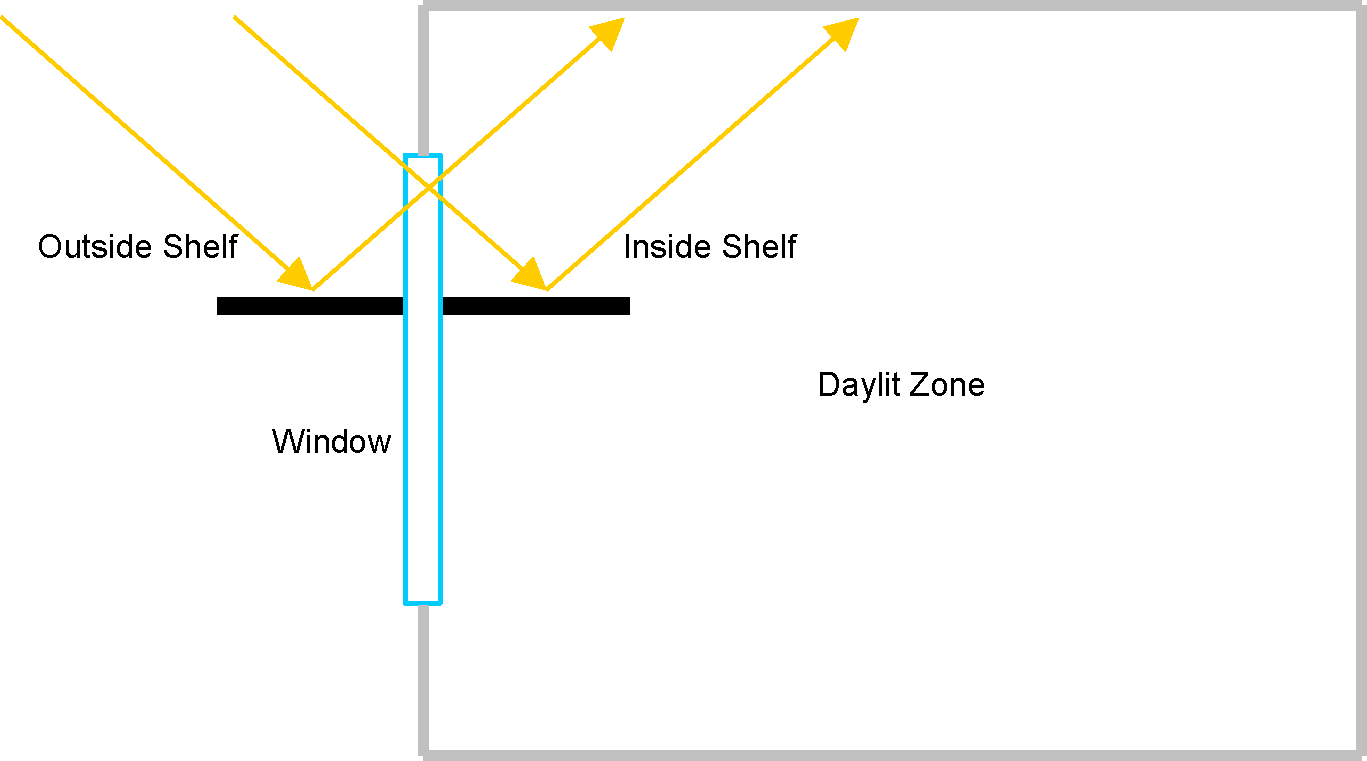
\includegraphics[width=0.9\textwidth, height=0.9\textheight, keepaspectratio=true]{media/image893.png}
\caption{Daylighting Shelf Diagram \protect \label{fig:daylighting-shelf-diagram}}
\end{figure}

Daylighting shelves are simulated separately for daylighting and the zone heat balance.~ The general model is similar in both cases, but the details vary.

\subsubsection{Inside Shelf Daylighting}\label{inside-shelf-daylighting}

The inside shelf is modeled in the daylighting simulation by converting all light transmitted by the upper window into diffuse upgoing flux.~ It is assumed that no beam or downgoing flux can pass the end of the shelf regardless of the shelf's position or orientation.

In the daylighting simulation this is accomplished by forcing all the transmitted flux to be upgoing:

\begin{equation}
{\Phi_{CW}} = \Phi
\end{equation}

\begin{equation}
{\Phi_{FW}} = 0
\end{equation}

where

\(\Phi_{CW}\) = upgoing flux

\(\Phi_{FW}\) = downgoing flux

\(\Phi\) = total flux

Since it is assumed that all light falls on the inside shelf, it is implied that the upper window~ cannot contribute any direct illuminance (i.e.~the upper window cannot be seen from anywhere in the zone).~ The remaining light is entirely interreflected sky-related and interreflected sun-related upgoing flux.

\subsubsection{Inside Shelf Heat Balance}\label{inside-shelf-heat-balance}

In the heat balance simulation the inside shelf is defined as an interzone heat transfer surface, e.g.~partition.~ Since the inside shelf external boundary condition is required to refer to itself, the shelf is essentially equivalent to internal mass.~ Because the shelf surface has two sides that participate in the zone heat balance, the surface area is doubled by the program during initialization.~ Like internal mass, the shelf surface is allowed to interact convectively and radiatively with the zone air and other zone surfaces.

The zone interior solar distribution is modified by the inside shelf.~ Regardless of the solar distribution selected in the input file, all beam solar radiation transmitted by the upper window is incident on one side (half the doubled surface area) of the shelf surface.~ The beam radiation not absorbed is reflected throughout the zone as diffuse shortwave radiation.~ The treatment of sky and ground radiation is unchanged; both are added directly to the zone diffuse shortwave.

The total beam, sky, and ground radiation transmitted by the upper window does not change.

\subsubsection{Outside Shelf Daylighting}\label{outside-shelf-daylighting}

In the daylighting model the luminous flux transmitted by the upper window is determined by integrating over the sky and ground and summing the luminance contribution of each sky or ground element.~ The luminance of any intervening exterior or interior surfaces is assumed to be zero.~ As a shading surface, the effect of the outside shelf during the integration is to block part of the view of the ground, thereby reducing the window transmitted flux due to diffuse ground luminance.~ After the integration is complete, the program calculates the amount of diffuse light that is reflected through the window from the outside shelf and adds it as a lump sum to the upgoing flux transmitted by the window.

The additional shelf upgoing flux is the sum of sun-related and sky-related flux:

\begin{equation}
{\Phi_{shelf,CW}} = {\Phi_{shelf,sun}} + {\Phi_{shelf,sky}}
\end{equation}

where

\begin{equation}
{\Phi_{shelf,sun}} = \left( {{E_{sun}}\cos \theta } \right){f_{sunlit}}{\rho_{vis}}{F_{ws}}{\tau_{diff,vis}}
\end{equation}

\begin{equation}
{\Phi_{shelf,sky}} = {E_{h,sky}}{f_{skymult}}{\rho_{vis}}{F_{ws}}{\tau_{diff,vis}}
\end{equation}

and

E\(_{sun}\) = exterior illuminance due to light from the sun

E\(_{h,\,sky}\) = exterior horizontal illuminance due to light from the sky

\(\theta\) = incident angle of the beam on the shelf

f\(_{sunlit}\) = sunlit beam fraction of the shelf surface area

f\(_{skymult}\) = anisotropic sky view multiplier (see AnisoSkyMult)

\(\rho_{vis}\) = shelf surface reflectivity in the visible spectrum

F\(_{ws}\) = view factor from window to shelf

\(\tau_{diff,\, vis}\) = diffuse window transmittance in the visible spectrum

The sunlit beam fraction f\(_{sunlit}\) and the anisotropic sky view multiplier f\(_{skymult}\) are borrowed from the heat balance solar calculations.

The sunlit beam fraction f\(_{sunlit}\) takes into account the effect of shading due to other surfaces.~ Although shadows on the shelf surface change the luminance distribution of the shelf, there is no angular dependence because diffuse properties are assumed.~ Therefore, the flux is simply proportional to the sunlit fraction.

The anisotropic sky view multiplier f\(_{skymult}\) takes into account the anisotropic distribution of sky radiation, the shelf view factor to the sky, and shading.~ This value is utilized in the heat balance simulation for solar calculations but is not currently available in the daylighting simulation.~ A value of 1.0 is assumed until a better model is developed.~ For this reason the sky-related flux may be over-predicted for some building and shelf geometries.~ However, for clear sky conditions the sun-related flux is dominant and the resulting error is small.

The view factor to the outside shelf, F\(_{ws}\), if not specified by the user in the input object, is an exact view factor calculated for adjacent perpendicular rectangles.

\begin{figure}[hbtp] % fig 71
\centering
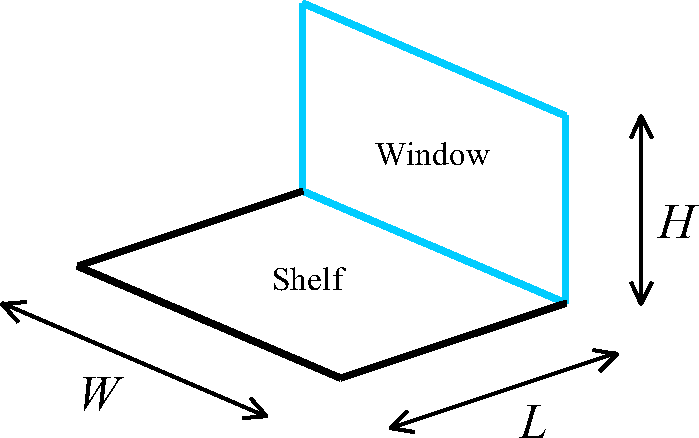
\includegraphics[width=0.9\textwidth, height=0.9\textheight, keepaspectratio=true]{media/image899.png}
\caption{Window and Outside Shelf as Adjacent Perpendicular Rectangles. \protect \label{fig:window-and-outside-shelf-as-adjacent}}
\end{figure}

For this geometry the view factor is given by (Mills 1995):

\begin{equation}
{F_{ws}} = \frac{1}{{\pi M}}\left\{ \begin{array}{l}M{\tan ^{ - 1}}\left( {\frac{1}{M}} \right) + N{\tan ^{ - 1}}\left( {\frac{1}{N}} \right) - {\left( {{M^2} + {N^2}} \right)^{1/2}}{\tan ^{ - 1}}\left( {{{\left( {{M^2} + {N^2}} \right)}^{ - 1/2}}} \right)\\ + \frac{1}{4}\ln \left[ {\left( {\frac{{\left( {1 + {M^2}} \right)\left( {1 + {N^2}} \right)}}{{1 + {M^2} + {N^2}}}} \right){{\left( {\frac{{{M^2}\left( {1 + {M^2} + {N^2}} \right)}}{{\left( {1 + {M^2}} \right)\left( {{M^2} + {N^2}} \right)}}} \right)}^{{M^2}}}{{\left( {\frac{{{N^2}\left( {1 + {M^2} + {N^2}} \right)}}{{\left( {1 + {N^2}} \right)\left( {{M^2} + {N^2}} \right)}}} \right)}^{{N^2}}}} \right]\end{array} \right\}
\end{equation}

where

\begin{equation}
M = H/W
\end{equation}

\begin{equation}
N = L/W
\end{equation}

\subsubsection{Outside Shelf Heat Balance}\label{outside-shelf-heat-balance}

The heat balance simulation does not do a sky and ground integration.~ View factors to sky and ground are used instead.~ Consequently, the heat balance calculation for the outside shelf is very similar to the daylighting calculation.~ The main difference is that the incident flux on the upper window is calculated first and reported.~ The transmitted and absorbed fractions are subsequently determined.

The solar flux incident on the upper window due to the shelf is given by:

\begin{equation}
{q''_{shelf - inc}} = {q''_{shelf - inc,sun}} + {q''_{shelf - inc,sky}}
\end{equation}

where

\begin{equation}
{q''_{shelf - inc,sun}} = \left( {{I_{sun}}\cos \theta } \right){f_{sunlit}}{\rho_{sol}}{F_{ws}}
\end{equation}

\begin{equation}
{q''_{shelf - inc,sky}} = {I_{h,sky}}{f_{skymult}}{\rho_{sol}}{F_{ws}}
\end{equation}

and

I\(_{sun}\) = solar beam intensity of the sun

I\(_{h,\, sky}\) = total horizontal diffuse solar radiation due to the sky

\(\theta\) = incident angle of the beam on the shelf

f\(_{sunlit}\) = sunlit beam fraction of the surface area

f\(_{skymult}\) = anisotropic sky view multiplier (see AnisoSkyMult)

\(\rho_{sol}\) = shelf surface reflectivity in the solar spectrum

F\(_{ws}\) = view factor from window to shelf

The view factor F\(_{ws}\) is the same as described above for daylighting.

The total diffuse incident radiation due to the shelf is internally added to the ground diffuse incident radiation on the window.~ For reporting purposes the shelf radiation is included in the \emph{Surface Outside Face Incident Ground Diffuse Solar Radiation Rate per Area} output variable.

With the incident radiation determined, the remaining window heat balance is calculated normally.~ The resulting transmitted diffuse radiation from the sky, ground, and shelf is:

\begin{equation}
{q''_{trans}} = \left( {{{q''}_{sky - inc}} + {{q''}_{gnd - inc}} + {{q''}_{shelf - inc}}} \right){\tau_{diff,sol}}
\end{equation}

where

\(\tau_{diff,\, sol}\) = diffuse window transmittance in the solar spectrum

\subsubsection{References}\label{references-1-006}

Mills, A. F. 1995. Heat and Mass Transfer, p.~499.

\subsection{Window Light Well}\label{window-light-well}

The input object DaylightingDevice:LightWell provides a model for attenuation of light transmitted by windows and skylights that can result from surrounding interior finish surfaces that form a ``light well.''~ The light well model simply attenuates the light transmitted by the exterior window.~ The model does not redirect light distributions or alter the relative mixture of diffuse and beam transmitted by the window.

The attenuation is characterized by the \textbf{well efficiency}, which is the ratio of the amount of light leaving the well to the amount of light entering the well. The well efficiency varies from close to 1.0~ to close to zero if there is high attenuation. The well efficiency is used only in the EnergyPlus detailed daylighting calculation, where it multiplies the beam and diffuse light transmitted by the skylight. (The well efficiency is not used in calculating the solar gain through the skylight.)

\begin{figure}[hbtp] % fig 72
\centering
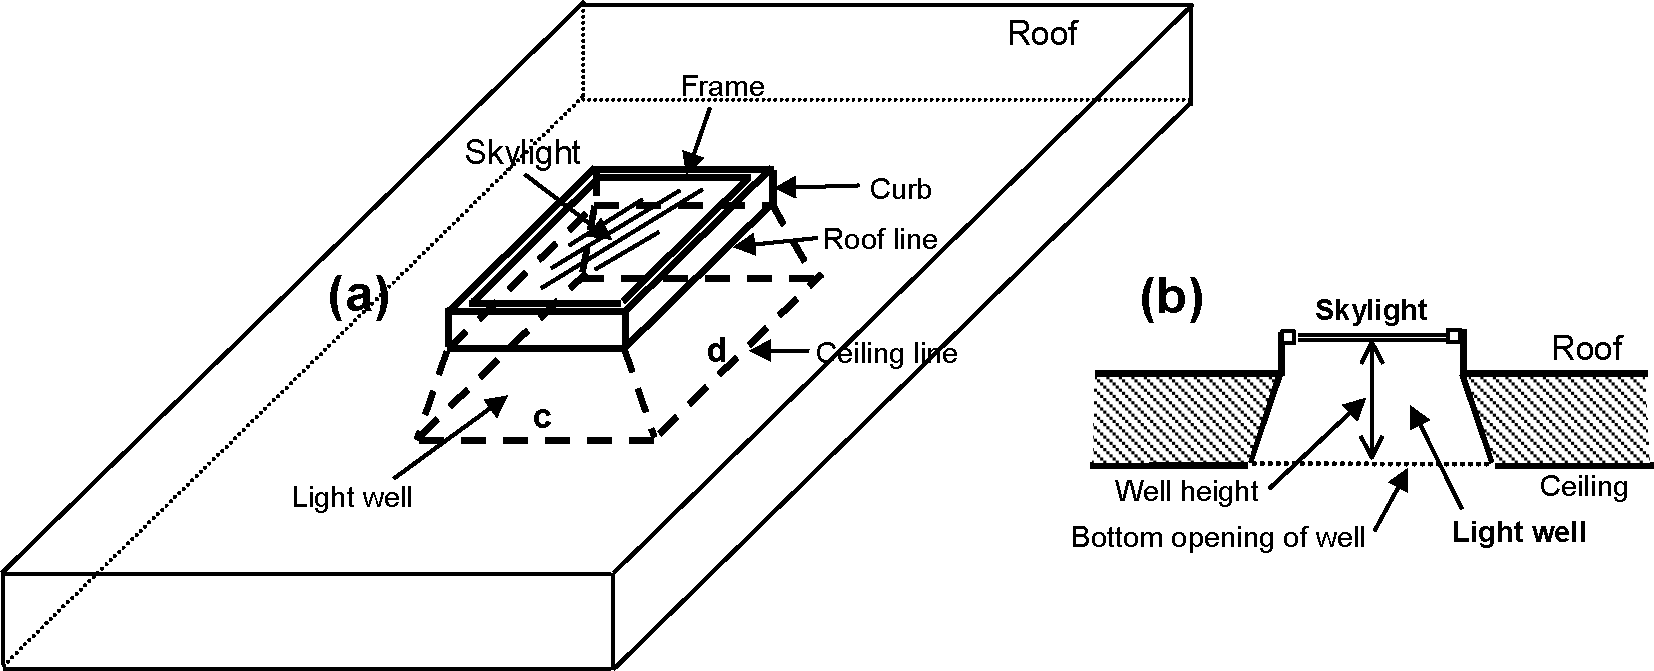
\includegraphics[width=0.9\textwidth, height=0.9\textheight, keepaspectratio=true]{media/image907.png}
\caption{Skylight with light well: (a) perspective view, (b) vertical section. If the bottom of the light well is a rectangle of side lengths c and d, as shown in (a), then the perimeter of the bottom of the well = 2(c+d) and the area = cd (see description of field names for the Light Well object). \protect \label{fig:skylight-with-light-well-a-perspective-view-b}}
\end{figure}

The well efficiency depends on the visible reflectance of well's side walls and on the well cavity ratio, \textbf{\emph{WCR}}, which is given by:

\begin{equation}
WCR = \frac{{{\rm{2}}{\rm{.5 x Well~Height x Well~Perimeter}}}}{{{\rm{Well~Area}}}}
\end{equation}

Well Height, Well Perimeter and Well Area are inputs to the model and are discussed in the figure caption above.

The model in EnergyPlus was implemented by fitting a curve to the data presented as Figure~8-21, ``Efficiency factors for various depths of light wells based on well-interreflectance values,'' found in the Lighting Handbook (IES 1993).~ The figure below reproduces that reference data and shows well efficiency vs.~WCR for different side wall reflectances. For use in the EnergyPlus calculation, a fit has been made to this graph that gives the following mathematical expression, where ``Reflectance'' is the user input value of the well-wall reflectance expressed as a fraction:

\begin{equation}
{\rm{Well~efficiency}} = {e^{ - WCR*(0.16368 - 0.144678*{\rm{Reflectance}})}}
\end{equation}

\begin{figure}[hbtp] % fig 73
\centering
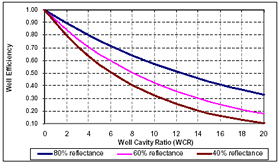
\includegraphics[width=0.9\textwidth, height=0.9\textheight, keepaspectratio=true]{media/image910.png}
\caption{Graph showing light well efficiency vs. well cavity ratio (WCR) for well-wall visible reflectances of 80\% (upper curve), 60\% (middle curve) and 40\% (lower curve). Based on Fig. 8-21 of the Lighting Handbook: Reference and Application, 8\(^{th}\) Edition, 1993, Illuminating Engineering Society of North America. \protect \label{fig:graph-showing-light-well-efficiency-vs.-well}}
\end{figure}

The well efficiency calculated using this curve fit and user inputs is then applied to daylight transmission rates to attenuate daylight as a result of the presence of the light well,

\subsubsection{References}\label{references-2-004}

Lighting Handbook: Reference \& Application, 8th Edition, Illuminating Engineering Society of North America, 1993.
